% This is the main document file, it references all chapers that can be found in the "chapters" folder
\documentclass[12pt, twoside]{scrreprt}

% Packages
\usepackage[babelshorthands]{polyglossia} % English language settings
\setdefaultlanguage[variant=british]{english}
\usepackage[autostyle=true,english=british]{csquotes} % Quotation marks with enquote
  \MakeOuterQuote{"} % Automatically transforms the `"` character to the right quotation marks
\usepackage[singlespacing]{setspace} % Einfacher Durchschuss/ Zeilenabstand
\usepackage[a4paper, total={7in, 9in}]{geometry} % 2,6 cm Seitenränder links und rechts
\usepackage{blindtext} % Lorem Ipsum 
\usepackage[toc, acronym]{glossaries}
\usepackage{scrhack} % Avoids warnings when using listings
\usepackage[draft=false]{microtype} % Better type setting
\usepackage[titletoc]{appendix} % Makes "appendix" appear in front of each appendinx in the toc
\usepackage{enumerate}  % for ordered lists
\usepackage[shortlabels]{enumitem} %... and their customization

% Schriftart Auswahl
\usepackage{fontspec}
\setmainfont{TeX Gyre Pagella} %palatino clone

% Package for monospaced code blocks
\usepackage{listings}
\lstset{
    basicstyle=\ttfamily,
    escapeinside={||}
}
\usepackage{amsmath}  % for \hookrightarrow // um zeileinumbrüche zu markieren
\usepackage{xcolor}   % for \textcolor

% Packages to embed images, svgs, pdf pages
% Draft
\PassOptionsToPackage{draft}{graphicx}
\usepackage[draft]{pdfpages} % Allows to embed PDF pages page-filling (using \includepdf)
% No Draft
% \PassOptionsToPackage{}{graphicx}
% \usepackage[]{pdfpages} % Allows to embed PDF pages page-filling (using \includepdf)

\usepackage{subcaption} % Combine multiple images into one figure with \subfigure
\graphicspath{{./images/}}
\usepackage[inkscapearea=page]{svg} % Doku https://ftp.fau.de/ctan/graphics/svg/doc/svg.pdf
\usepackage{relsize} % um schriftgrößen innerhalb eines svgs relativ zueinander anzupassen
\svgpath{images/}


% Package for active hyperlinks for references and inside the biliography
\usepackage{bookmark} % Included hyperref automatisch
\hypersetup{
  colorlinks   = true, %Colours links instead of ugly boxes
  urlcolor     = blue, %Colour for external hyperlinks
  linkcolor    = blue, %Colour of internal links
  citecolor   = red, %Colour of citations
  pdftitle = Team We Want a Toast Group 1 - Assignment WS 22/23,
  pdfauthor = Laurenz Bihlmayer,
  plainpages=false,
  bookmarksnumbered=true,
  bookmarksopen=true,   % Opens all pdf bookmarks until level 1 (section)
  bookmarksopenlevel=1,
}


% Header and footer with Scrlayer-Scrpage
\usepackage[headsepline]{scrlayer-scrpage}
\pagestyle{scrheadings}
\clearpairofpagestyles

% Show the current title and chapter on the top of each (double) page
\ohead{\headmark}
\automark[section]{chapter} %[right side]{left side}
\ofoot*{\pagemark} %Page number in the footer

% Bibliography
\usepackage[style=authoryear-ibid, sorting=ynt, maxcitenames=2 ]{biblatex}
\setcounter{biburllcpenalty}{7000}
\setcounter{biburlucpenalty}{8000}
\addbibresource{references.bib}

% Glossary
\makeglossaries

% Glossar
\newglossaryentry{subversion}{
    name={Apache Subversion},
    description={Apache Subversion ist ein zentrales Open-Source Versionskontrollsystem}
}




% Akronyme
\newacronym{png}{PNG}{Portable Network Graphics}

\newacronym{svg}{SVG}{Scalable Vector Graphics}

\newacronym{json}{JSON}{JavaScript Object Notation}




\begin{document}

% Titlepage
\pagenumbering{Roman}
\hypertarget{titlepage}{}% set the hypertarget
\bookmark[dest=titlepage,level=chapter]{Title page}% add the bookmark

\newgeometry{top=3cm,bottom=3cm}
\begin{titlepage}

    \begin{center}
        \large
        University of Cologne\\
        Faculty of Management, Economics and Social Sciences 

        \vspace*{1cm}
        \large
        San Francisco 2019

        \Huge
        \textbf{Team \enquote{We Want a Toast}\\ Group 1 - Assignment WS 22/23 }

        \vspace{1.5cm}
        \large
        For the study program Information System 
        \vspace{0.8cm}
    \end{center}

    \vfill

    \begin{flushleft}
        \normalsize
        \begin{tabbing}
            ~~~~~~~~~~~~~~~~~~~~~~~~~~~~~~~~~~~~~\=\\ \kill % This line is not printed, it is just to  set/ fill the width until the first tab stop appears using the unprinted char `~'
            Authors: \>Laurenz Bihlmayer\\ 
            \>Leo Niggemann\\
            \> Manuel Heeren\\
            \> Tobias Wißmach\\\\

            Repository Link:\>\url{https://github.com/major-mayer/aawewantatoast}\\\\
    
            Lecture:\>Analytics and Application \\
            Instructor:\>Prof. Dr. Wolfgang Ketter \\ 
            Submission date:\>31.01.2023\\
        \end{tabbing}
   
    \end{flushleft}

\end{titlepage}
\restoregeometry


% Abstracts 
% Sorgt für eine korrekte Anzeige im PDF Index
\hypertarget{abstract}{}
\bookmark[dest=abstract,level=chapter]{Abstract}

\thispagestyle{plain}

\begin{center}
    \LARGE{\textbf{Executive summary}}
\end{center}

The main objective of this project was to analyze trip data from Lyft's bike rentals in San Francisco for the year 2019 in order to monitor and predict demand. To achieve this, we used three data sets that were cleaned and joined together; these included bike rental data for San Francisco, weather data for 2019 from weather.com, and geodata provided by Lyft's system data for the bike stations. Additionally, we established key performance indicators (KPIs) to monitor the operational performance of the bike fleet.

Through cluster analysis, we were able to gain a deeper understanding of the customer groups and station relevance. We found the following customer groups: \enquote{Nightriders}, which mainly ride in the early morning and late evening hours,  the "Workers" which take a bike to commute to work and lastly the "Midday rides". 

Our findings also showed that the highest demand for bike rentals occurred during the weekday morning and evening rush hours, with the busiest bike stations located in downtown San Francisco. 
Lastly, we implemented a predictive analysis to forecast demand and optimize the performance of the fleet in the future. For the model, we chose the K-Nearest-Neighbor model, because it showed the best R² value of 0.956773. We also found out, that the lag feature from one week before as well as the \texttt{is\_workday} feature are the most important features for the prediction.

To optimize the performance of the fleet, we recommend that Lyft focus on increasing the availability of bikes at these busy stations during peak hours, as well as providing promotions and incentives for both short-trip and weekend-customers. Additionally, our analysis revealed the existence of two customer clusters: short-trip customers who primarily use bikes for commuting purposes, and weekend-customers who use bikes for leisure and recreation. To better serve these customers, Lyft should consider offering corporate subscriptions for short-trip customers and promotions for long-trip customers on weekends.

The results of our analysis are based on a limited dataset, which includes only one year of bike rental data and lacks information on user demographics and user distinction as distinction. Nevertheless, our findings and recommendations provide a solid foundation for Lyft to improve its bike-sharing service and better meet the needs of its customers.


% Table of content
\microtypesetup{protrusion=false}
\hypertarget{tableofcontents}{}% set the hypertarget
\bookmark[dest=tableofcontents,level=chapter]{\contentsname}% add the bookmark
\tableofcontents
\microtypesetup{protrusion=true}

% List of figures
% Two command to make sure the link doesn't point to the start of the section (table of contents)
\clearpage
\phantomsection
\addcontentsline{toc}{chapter}{List of figures}

\microtypesetup{protrusion=false}
\listoffigures
\microtypesetup{protrusion=true}

% Real content
\cleardoublepage % A clear double page in front of the page
\pagenumbering{arabic} % Wechsel des Nummerierungsstils auf arabische Ziffern

\section{Problem Description}

The fundamental goal of this project is to inform and improve business decisions for the bike-sharing platform Lyft. By conducting analysis on historical data, we aim at identifying patterns and trends that unfold demand-driving factors and thereby enhance allocation. To gain a more comprehensive understanding of these behavioural patterns, we generate costumer, time and spatial based clusters and provide hourly demand forecasting.
\chapter{Data Description and Preparation}
To conduct the data analysis, we utilized the following data sets: \href{run:../../data/sf_2019.csv}{sf\_2019.csv}, \href{run:../../data/weather_hourly_sf.csv}{weather\_hourly\_sf.csv}, and \href{run:../../data/Sf_2019_full.csv}{Sf\_2019\_full.csv}. In the following section, we will provide an overview of the data and explain the steps we took to prepare it.

\section{Ride Data}
The data for the bike rides is located in the \href{run:../../data/sf_2019.csv}{sf\_2019.csv} file and includes 2,506,982 trips that were taken in San Francisco in 2019. The file provides us with information about the start and end time, start and end station, as well as the user type, which can be either a subscriber or a customer. 

\begin{figure}[h]
    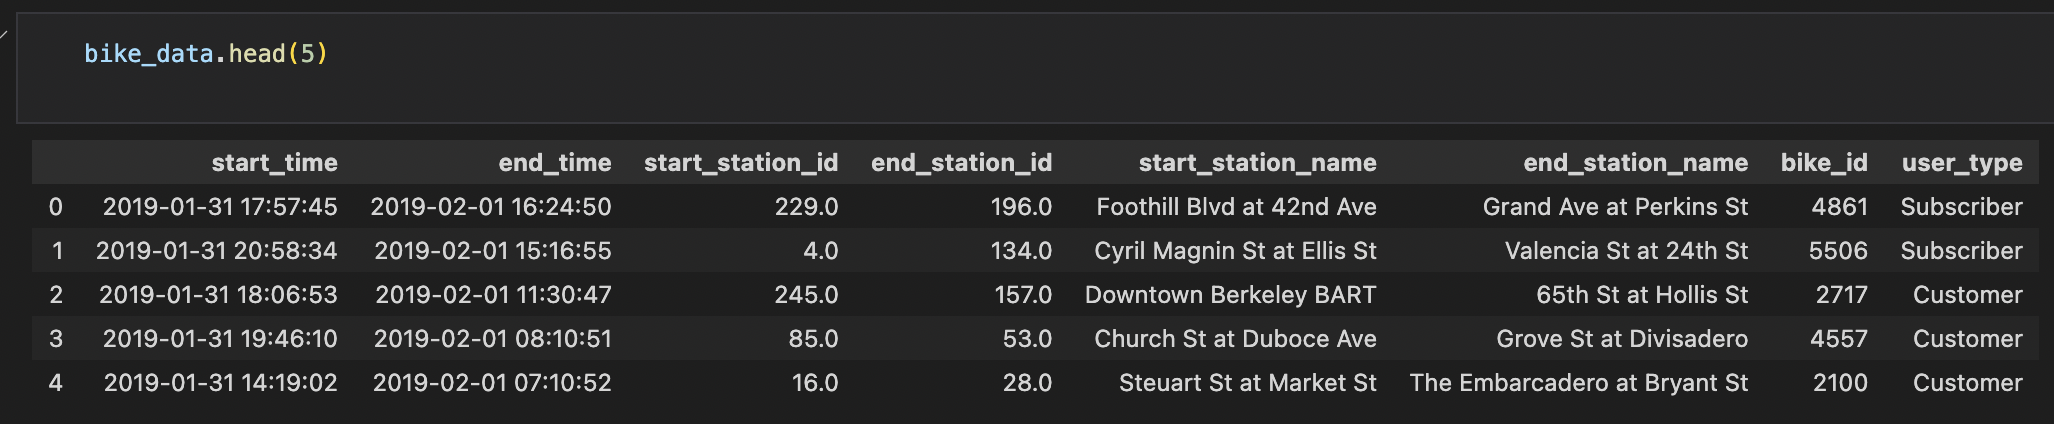
\includegraphics[width=\textwidth]{descriptive_rides.png}
    \caption{An excerpt from the trip dataset.}
    % \label{fig:png}
\end{figure}

In the first step, we examined the data for missing or incomplete values, and any duplicate entries. Thankfully, we did not find any duplicate values.

To improve our further analysis, we then added additional features to the dataset such as numeric features for \texttt{start\_hour}, \texttt{start\_weekday}, \texttt{start\_month} as well as the \texttt{trip\_duration} measured in seconds.

We then combined the external data set \href{run:../../data/Sf_2019_full.csv}{Sf\_2019\_full.csv} with the trips data set. Therefore, we created a look-up table including the \texttt{station\_id} as well as the station's actual geo coordinates from external data set and joined the geo data on the original trip data set. 
The enhanced geo features allowed us to refine the dataset to only include data from stations located in San Francisco. Trips with empty \texttt{station\_id} values are assumed to happen within the San Francisco area. That applies to around 3 \% of all trips and has a noticeable impact on the overall demand. We also removed any trips with suspicious data constellations in the trip duration as negative trip durations or outliers. We eliminated the top 0.5\% of trip durations, which were all trips that lasted longer than two hours. 

\section{Weather Data}
% added column names and the necessary time shift to match the trip data
The file \href{run:../../data/weather_hourly_sf.csv}{weather\_hourly\_sf.csv} gives us information about the weather in San Francisco in 2019. It includes the columns \texttt{date\_time}, \texttt{max\_temp}, \texttt{max\_temp} and the precipitation \texttt{precip}. The values of \texttt{date\_time} are UTC timestamps and needed to be shifted by -8 hours to match the ride data.

\begin{figure}[h]
    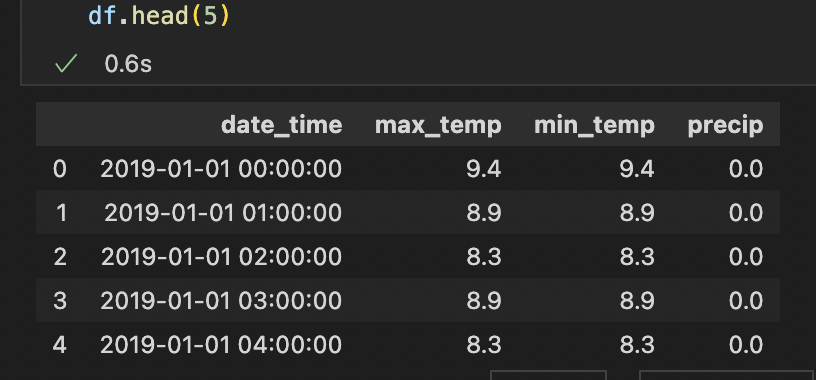
\includegraphics[width=\textwidth]{descriptive_weather.png}
    \caption{An excerpt from the weather dataset.}
    % \label{fig:png}
\end{figure}

For weather data cleaning, we checked for any missing values or duplicate entries, similar to the process used for the rides data set. We did not find any missing values, but 79 duplicate rows across all columns of the data frame and 371 duplicate entries in the \texttt{date\_time} column.

As we did not want to drop any columns easily, we determined the ratio of hourly temperature changes across the entire dataset. Temperature changes on an hourly basis at odds of roughly 2:1. The duplicated rows in the data frame can therefore be a result of duplicated entries in the \texttt{date\_time} column co-occurring with a natural steady temperature trend.
Since temperature values tend to not change within the course of an hour in non-duplicates as well, we did not declare the duplicates as redundant data. Instead, we kept the entries but adjusted the \texttt{date\_time} column by shifting these timestamps forward until no \texttt{date\_time} duplicates remain. Dropping duplicates and interpolating new values was not necessary.
\section{Data Analysis}

\subsection{Descriptive Analysis}
\subsubsection{Temporal Demand Patterns} 

We aggregated the variable time on the different hierarchy levels month, weekday and hour. The monthly demand shows no clear trend, probably due to low temperature variation between the seasons in San Francisco. On weekends there is less demand, indicating that bike usage is mainly for trips to and from work. This assumption is supported by the hourly demand patterns. Peaks are at the morning hours around 8am and at around 5pm. Between 1am and 5am, demand is at a minimum. 

\begin{figure}[hbtp]
    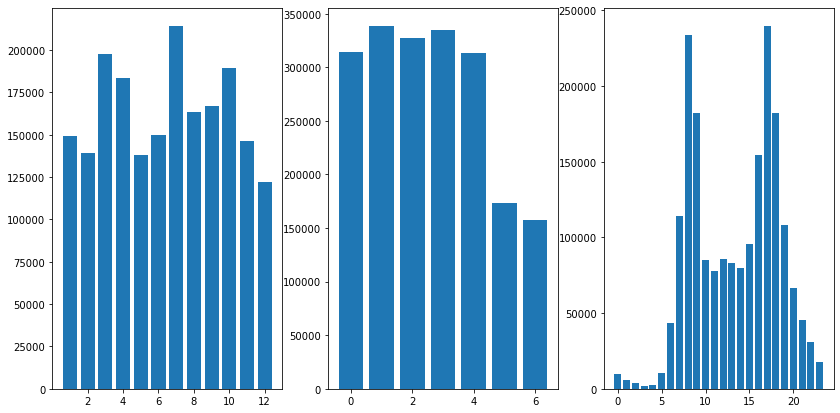
\includegraphics[width=\textwidth]{rides_plotted.png}
    \caption{Ride counts plotted on monthly, weekday, and hourly basis (from left to right).}
    % \label{fig:png}
\end{figure}

To investigate the weather dataset we plotted the average temperature over the hierarchy levels month, weekday and hour. The average temperatures get to a maximum of 19 °C in July and August and drop to a minimum of 10 °C in February. The demand pattern follows no clear temperature pattern, since there are maxima in demand in March and April. The mild climate in San Francisco seems to have no influence on the demand since the temperature range allows bike trips all year long.

\begin{figure}[hbtp]
    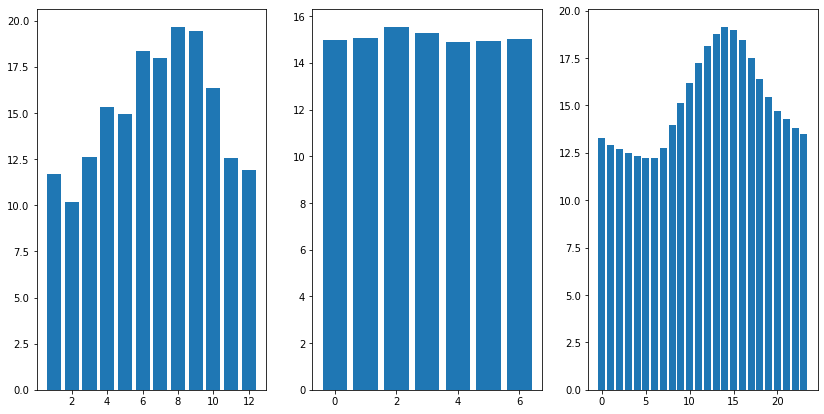
\includegraphics[width=\textwidth]{weather_plotted.png}
    \caption{Temperatures plotted on monthly, weekday, and hourly basis (from left to right).}
    % \label{fig:png}
\end{figure}

The heat map displays weekly trips through the combination of weekday and hour dimensions. It highlights that weekdays are busier than weekends during the peak commuting hours of 8 am and 5 pm, possibly indicating the presence of people traveling to work.

\begin{figure}[hbtp]
    \centering
    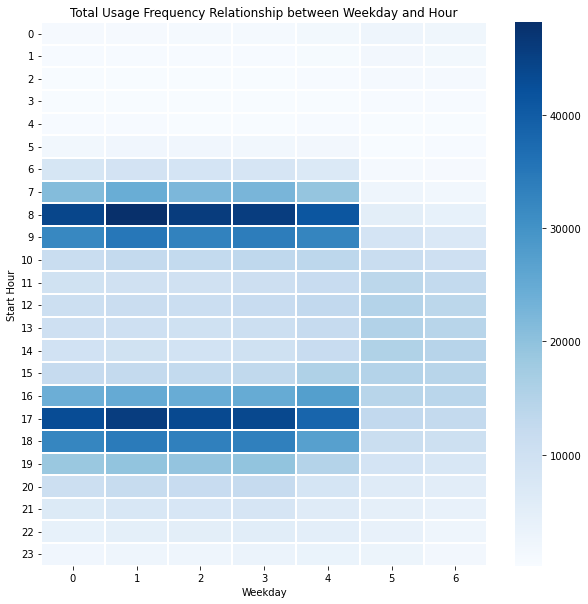
\includegraphics[width=0.5\textwidth]{rides_heatmap.png}
    \caption{Heat map that shows the relation between weekday (x-axis), hour (y-axis) and trip count (colour).}
    % \label{fig:png}
\end{figure}


\subsubsection{Geographical Demand Patterns}

The heatmap plots geographical locations of stations by latitude and longitude. Stations that are used frequently are yellow to red, and stations used sparsely are coloured purple. The main activity takes place at daytime in downtown San Francisco, more specifically in Valencia Street and Market Street. Other frequent stations are located around King Street and the docks. At nighttime stations are less frequently used and turn purple or disappear from the map. Interactive use of the heatmap is not possible via PDF, but with the notebooks in the repository that is linked. 

Plotting the monthly interactive Heatmap shows that trips taken at the beginning of the year are more centralized and trips taken towards the end of the year spread across a greater area, especially in the western city.

\subsubsection{Key Performance Indicators (KPIs)}

To monitor the fleet operations from a management perspective, we introduced the following KPIs:

First, we investigate the ratio of trips taken by subscribers and non-subscribers to differentiate between these pricing models. The average share of trips taken by subscribers across the whole dataset is around 79\%. Towards the end of the year, the ratio drops significantly. 

To answer the question of how often it is necessary to relocate a bike in a given time interval, we introduced the "Relocations" KPI. Therefore, we compared end stations to subsequent start stations to determine if relocations occurred. There is a peak of relocations at the end of July that could be potentially due to maintenance efforts.

\begin{figure}[hbtp]
    \centering
    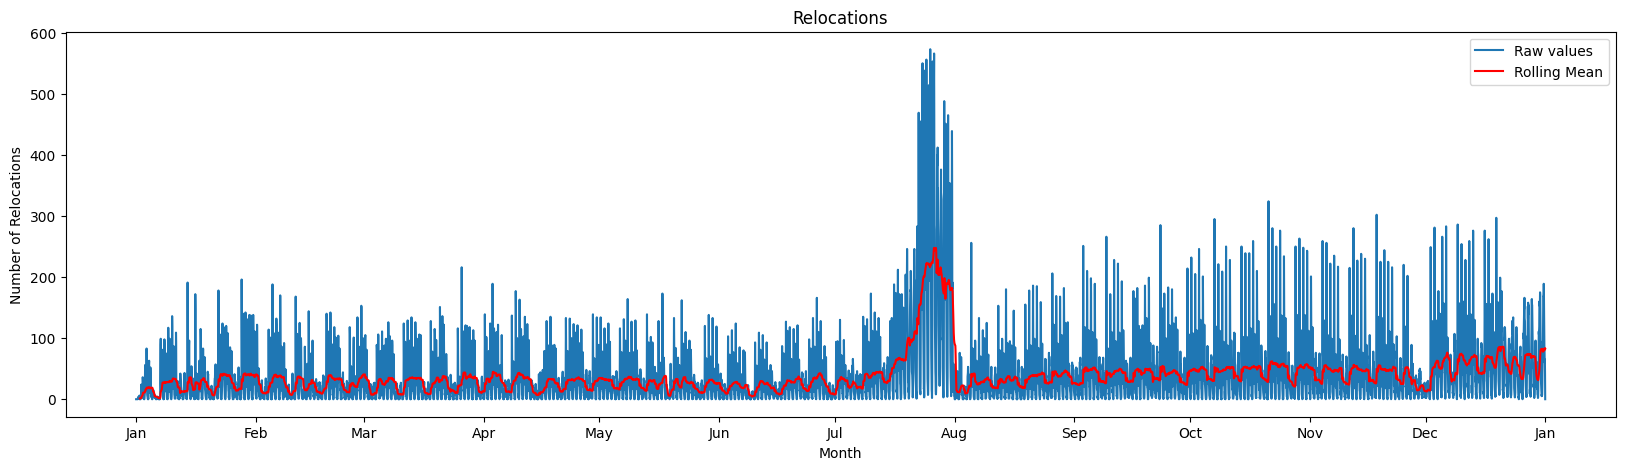
\includegraphics[width=\textwidth]{relocations.png}
    \caption{Plot that shows the number of relocations per hour.}
    % \label{fig:png}
\end{figure}



Our third KPI shows the distinct bikes in use per hour. On average, there are around 200-300 bikes in use per hour. Furthermore, the weekday patterns are identifiable. The peak at the end of July could be related to the peak of the "Relocation" KPI. To monitor the distribution we compared trips taken with distinct bikes. Values close to zero indicate a bad distribution of the bikes, whereas values near to one mean that the number of bikes used and trips taken is almost identical and thus indicate a good distribution of the bikes.

As our fourth KPI, we chose the revenue per hour. On average, Lyft has a revenue of about 900 USD per hour in San Francisco. The range of revenue per hour lies between a minimum of 3.49 USD and a maximum of 5760 USD. 

We only show the plot for the number of relocations here as an example. You can find all the other plots in the script.
\subsection{Cluster Analysis}

\subsection{Trip Clustering} 
Our trip clustering was based on the features \texttt{start\_hour}, \texttt{start\_weekday}, \texttt{start\_month}, \texttt{is\_weekend}, \texttt{user\_type} and  \texttt{trip\_duration}. Method wise we used the k-means clustering approach since it guarantees convergence and it 
scales to large datasets. On the downside we had to choose k the number of cluster manually. Therefore, we did a grid search to identify the elbow. After comparing k=3 and k=4 clusters we preferred to set k=3, because additional cluster mainly just split the \texttt{user\_type} in two different daytime clusters. The 3 resulting clusters all were sufficient in size and easily distinguishable, leading to a high content of information per cluster.


\begin{enumerate}[start=0]
    \item "Early Rides to work": Customers are characterized by a short trip duration compared to Cluster 1. They are taking trips in the typical
    work hour pattern described in the analysis section, but only in the morning hours. The cluster size of Cluster 0 and Cluster 2 are evenly distributed.
    \item "Weekend rides": Weekend rides are distinguishable by their weekday distribution, taking trips exclusively on weekends. Users on weekends
    are taking less short rides and longer trips, assuming that these are related to leisure activities. In terms of customer type the distribution shows no large deviation to the
    customer trip ratio of around 79\% across the whole dataset.
    \item "Late rides from work": The most distinctive feature is the time of day as of cluster one, but including only evening hours. Their subscriber share resembles
    the one of cluster 1 related to typical working hours, with only weekdays being included in the cluster as well.
\end{enumerate}

Analyzing the clusters created by K-Means algorithm, we presumed that the monthly feature is of less distinctive character, what was confirmed in
the predictive analysis.

\begin{figure}[hbtp]
    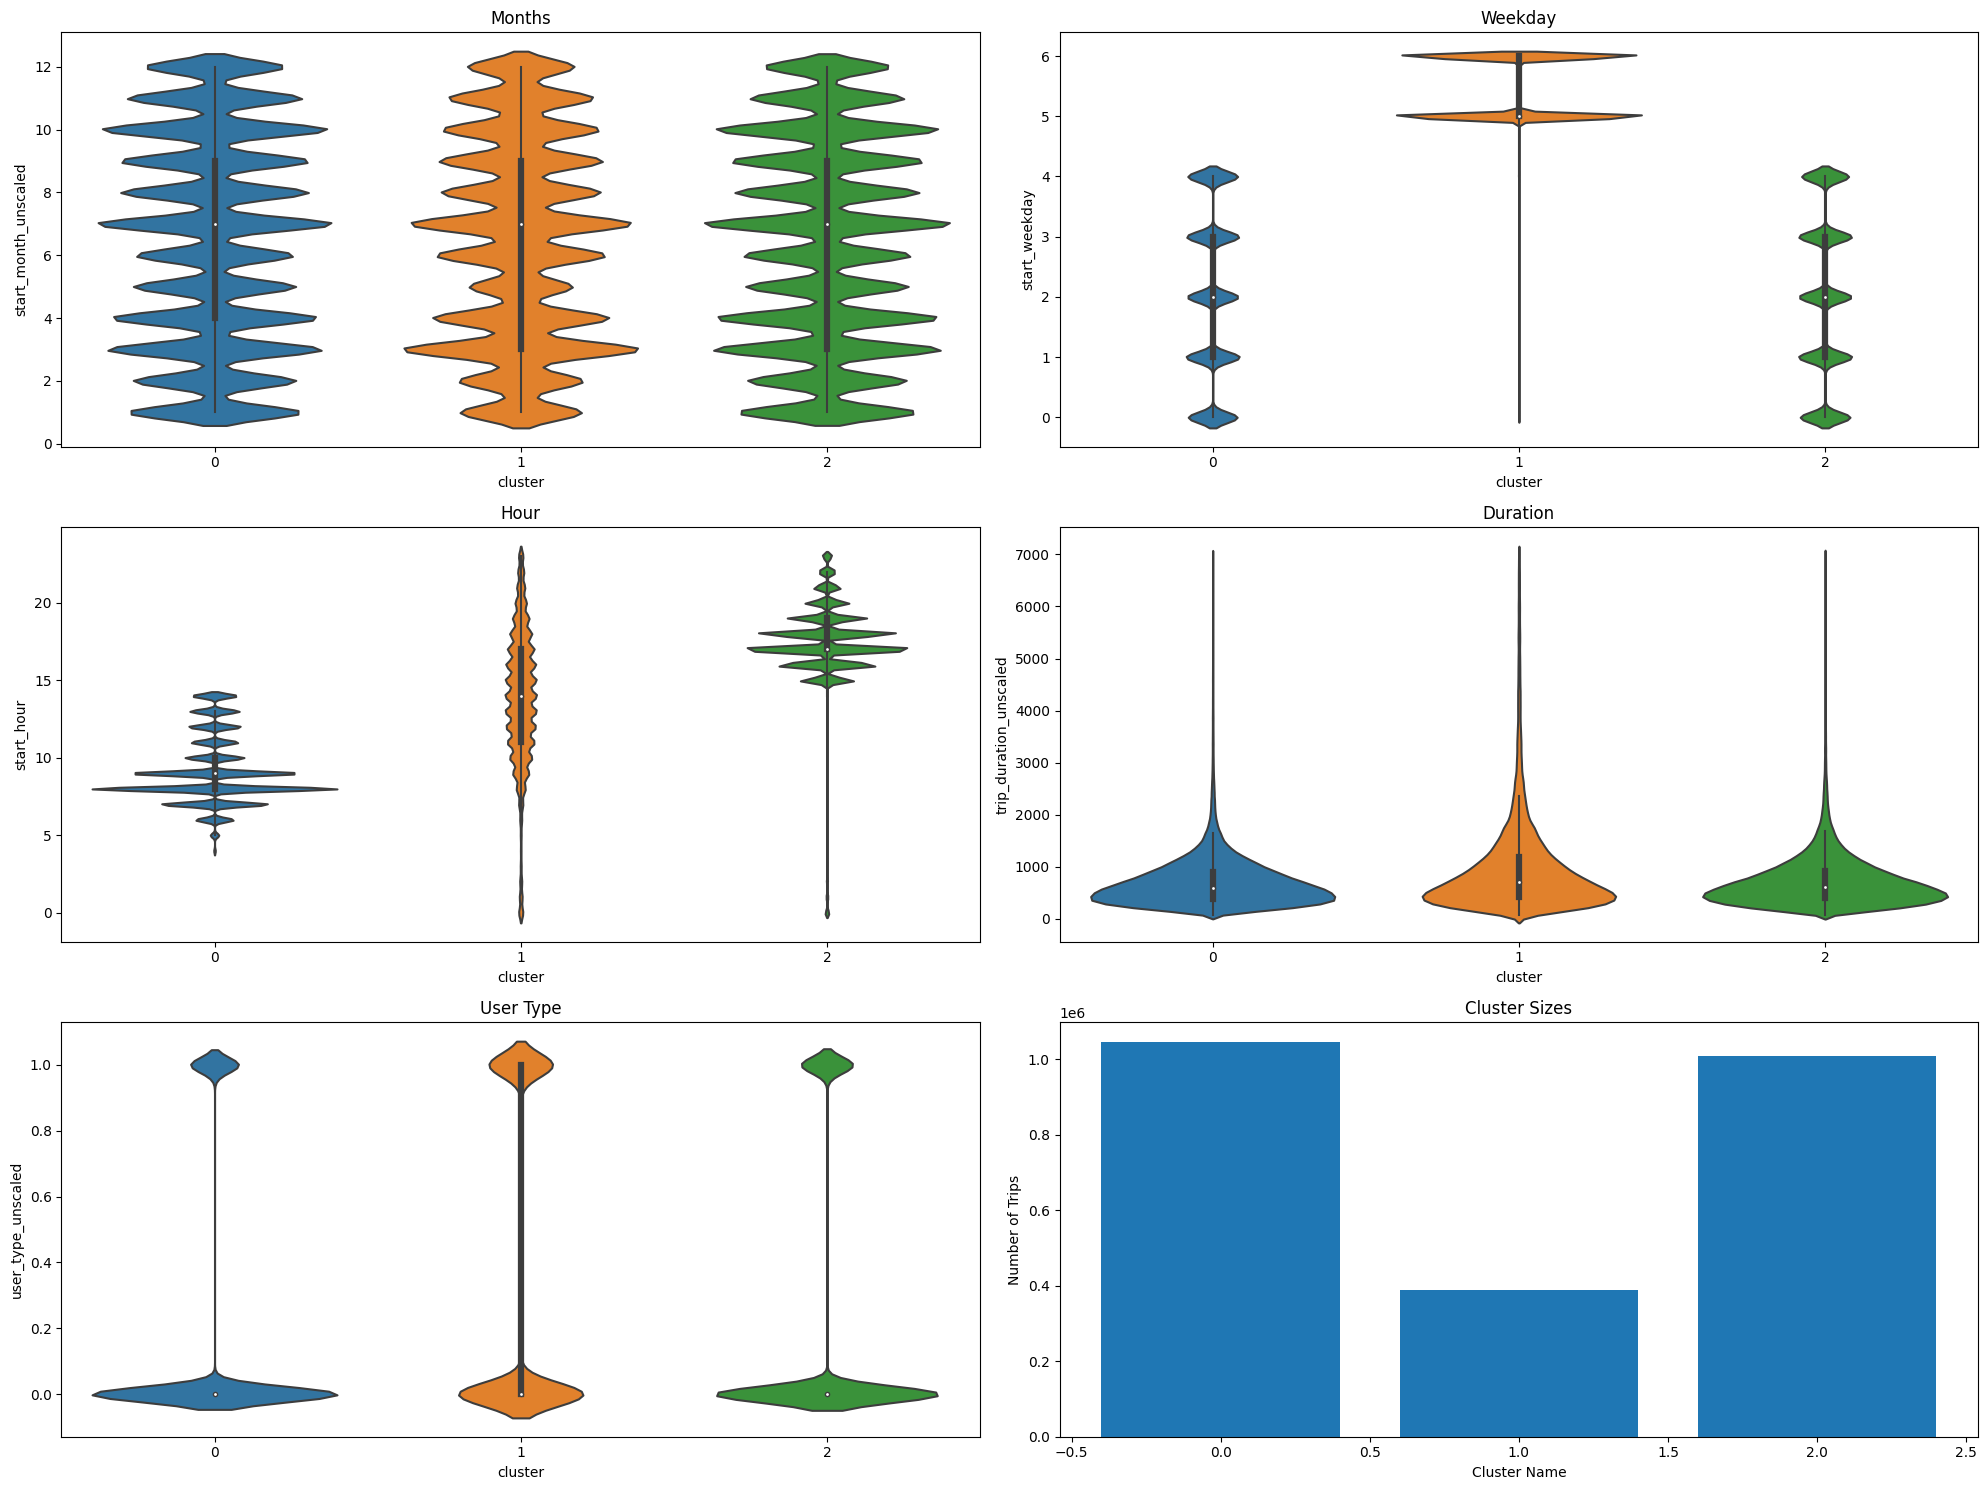
\includegraphics[width=\textwidth]{rides_cluster.png}   
    \caption{Trip clustering based on start\_month, start\_weekday, start\_hour, user type, trip duration and workday/weekend.}
    % \label{fig:png}
\end{figure}

\subsubsection{Weather Clustering}
The following features were used for K-Means Weather Data Clustering: precipitation, maximal temperature, months, weekday and hour. And we identified for k = 3 the clusters:

\begin{enumerate}[start=0]
    \item "Nightriders": Cluster 0 has a greater share of rides with precipitation and a lower average temperature. Rides are distributed around early morning hours and late evening hours when temperatures are obviously lower. 

    \item "Workers": This cluster reconstructs the work and weekday patterns of the trip clustering. Temperature wise, the cluster is evenly distributed.
 
    \item "Midday rides": Cluster 2 has the highest average temperature and rare precipitation. Trips are taken around midday more often compared to the other clusters. There is no weekday variation. 
\end{enumerate}

\begin{figure}[hbtp]
    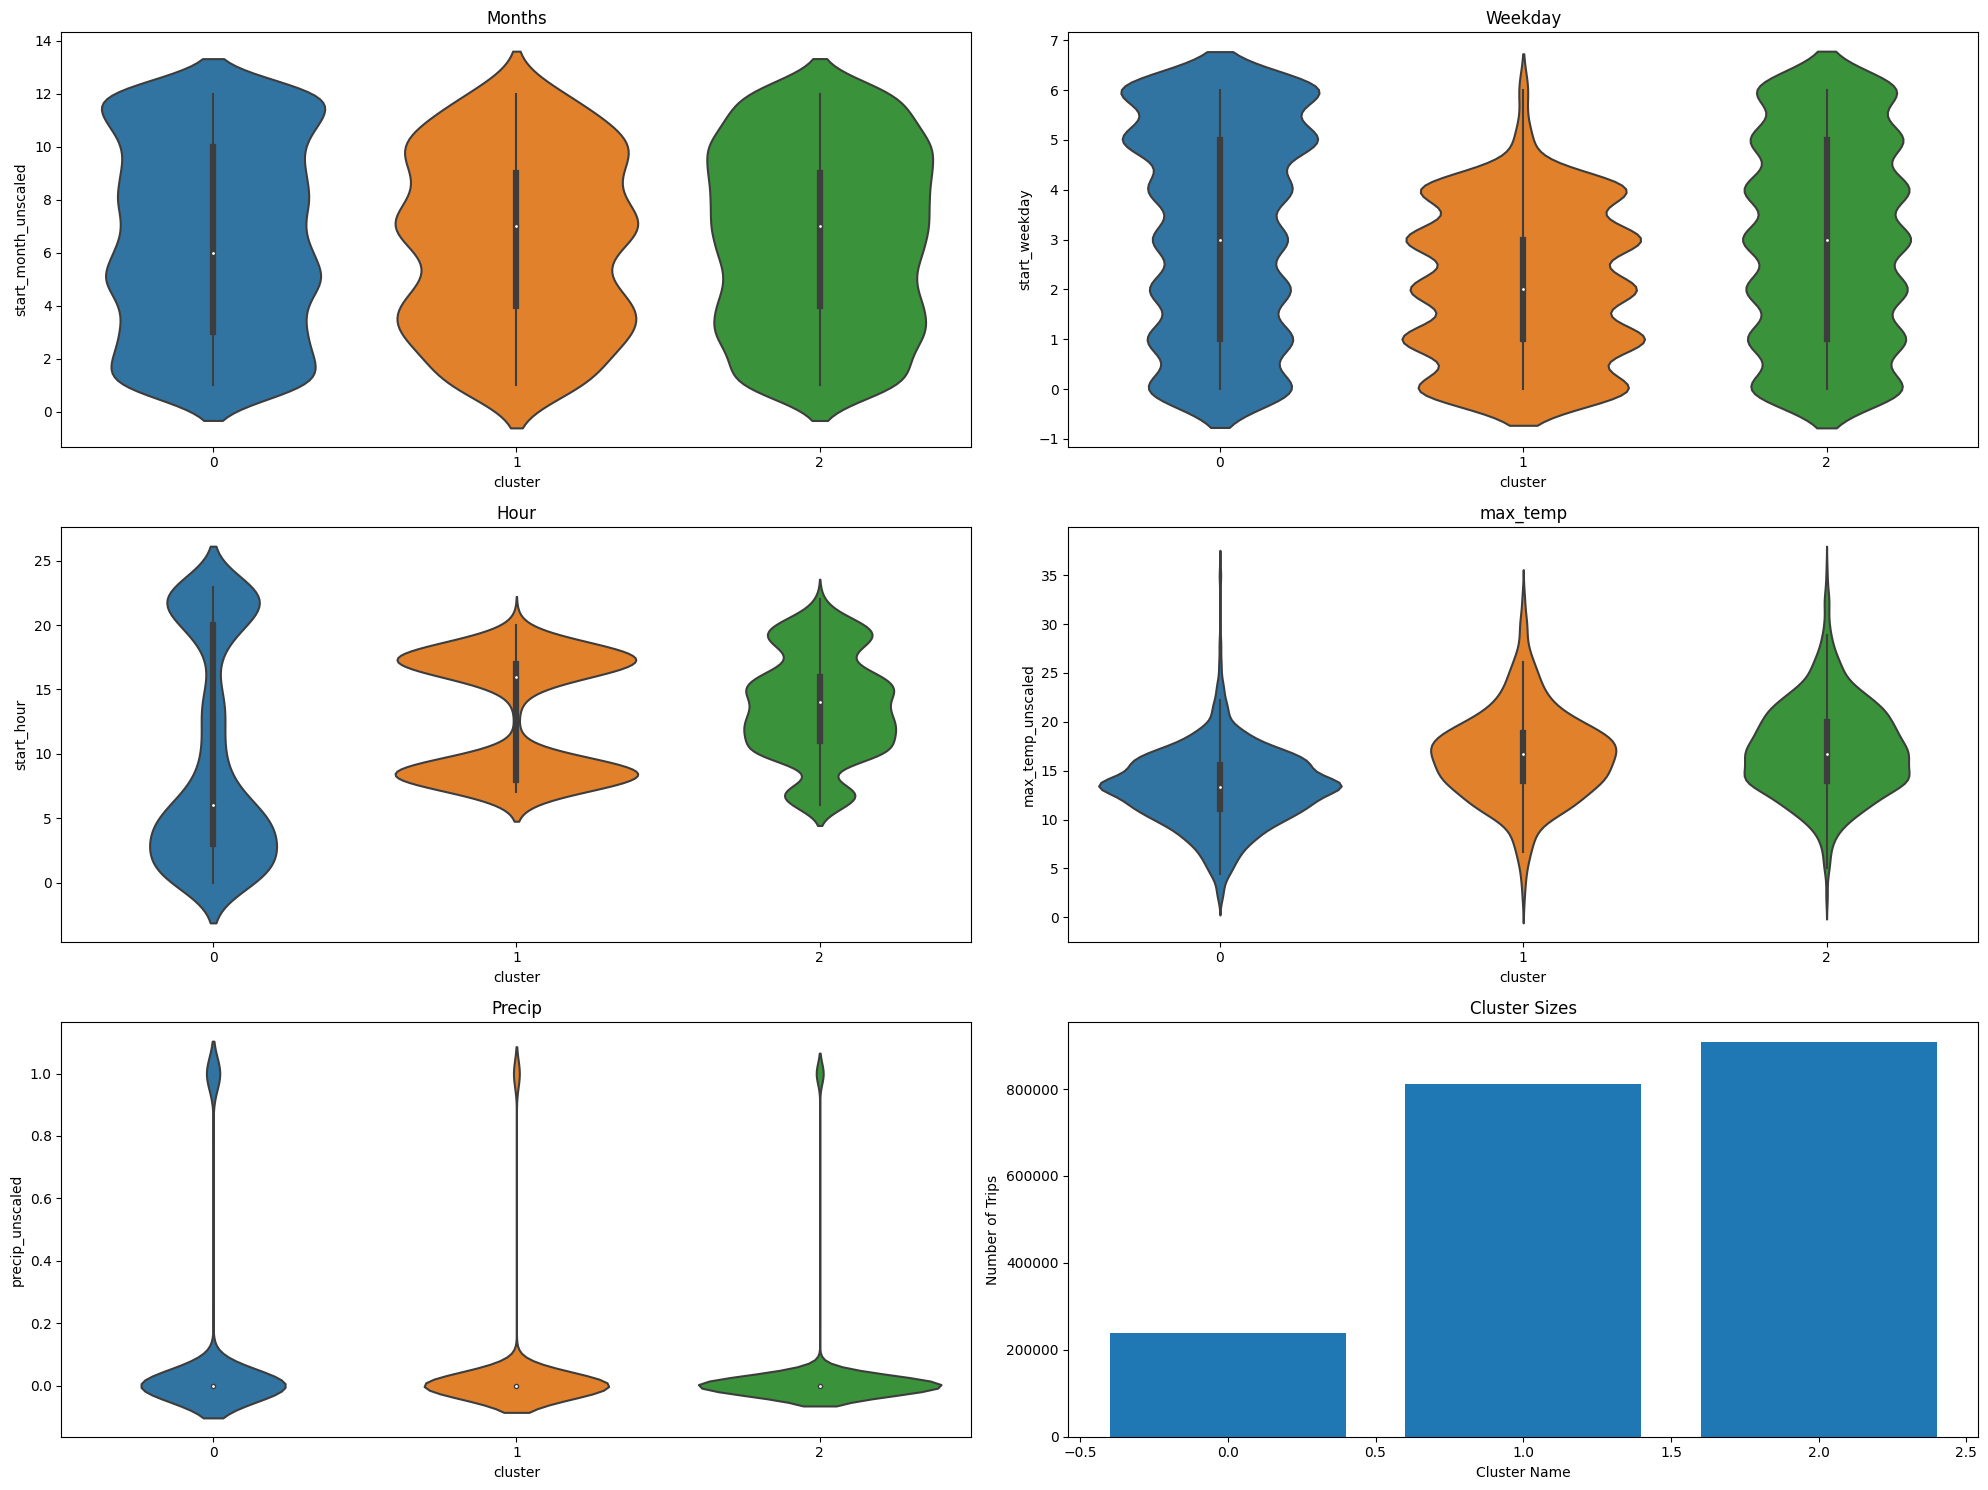
\includegraphics[width=\textwidth]{weather_cluster.png}
    \caption{Weather clustering based on month, weekday, hour, max. temperature and precipitation.}
    % \label{fig:png}
\end{figure}

The clustering of the weather data shows once again that neither temperature nor precipitation have a significant influence on demand. The identified clusters rather describe temporal correlations.

\subsubsection{Station Clustering}

The station clusters are computed based on location and usage. Therefore, they show the stations that are heavily frequented, less frequented and an in between cluster. As described in the Geographical Data Analysis, there are stations that can be characterized by being used less frequent and being distributed across a large area. These are grouped together in the cluster called "Low Performer". The "High Performer" - cluster are exactly the stations along the market street together with the eastern stations close to the docks. These are the stations that are frequented the most. Stations in the "Medium Performer" - Cluster are located mainly in downtown as well, but spread around a greater area than the "High Performer" - Cluster. These stations are also popular, but not as popular as the "High Performers" 

\begin{figure}[hbtp]
    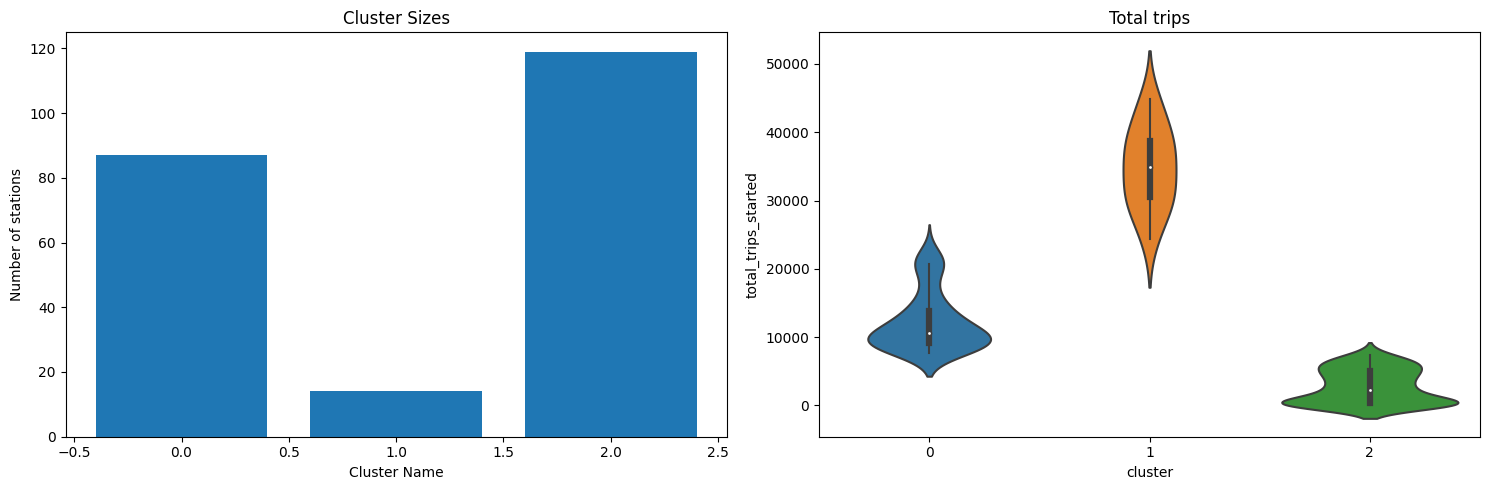
\includegraphics[width=\textwidth]{station_cluster.png}
    \caption{Station clustering based on location and usage.}
    % \label{fig:png}
\end{figure}


\subsection{Predictive Analysis}

\subsubsection{Preparation}
First, we created a small data set for predicting the hourly usage of the bike fleet. Bike trip data is aggregated, and the hourly demand is calculated. Location data is not part of the \texttt{prediction\_df} since the hourly demand of the whole bike fleet needs to be determined. Information on station granularity is therefore not considered. The weather data is reduced to the columns \texttt{max\_temp} and \texttt{precip}. 

\subsubsection{Feature Engineering}
We added additional features based on the analysis and clustering. Since a significant temporal correlation was discovered, these are for example seasonal features and lag features. We displayed the correlation of these features in the correlation matrix. We used a high correlation with the feature 'number\_of\_trips' for assessing features. 

\subsubsection{Grid Search Validation and Train/ Test Splitting}
To find the best combination of parameters for our models, we are using \texttt{GridSearchCV}.  It executes an exhaustive search over all parameters. \texttt{GridSearchCV} splits the data into multiple training and test sets with the same percentage of samples (cross validation). By default, the `KFold` algorithm is used which assumes independent samples and is not suitable for our time series dataset. This is because time series data always has the same sort of dependency to data from the past.

\begin{figure}[hbtp]
    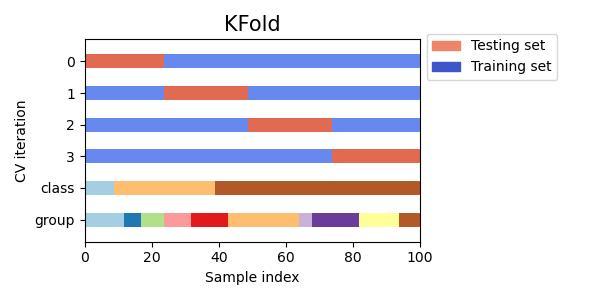
\includegraphics[width=0.49\textwidth]{kfold_algorithm.png}
    \hfill
    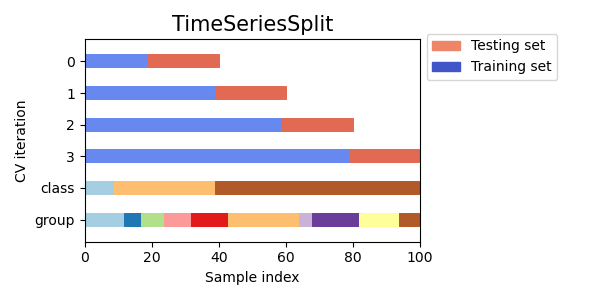
\includegraphics[width=0.49\textwidth]{timeseriessplit_algorithm.png}
    \caption{\texttt{KFold} and \texttt{TimeSeriesSplit} Algorithm. Source: \url{https://scikit-learn.org}}
    \label{fig:cv}
\end{figure}
 
As shown in the graph \ref{fig:cv}, the \texttt{KFold} algorithm would not ensure that the model works only on training data, instead, we are using the \texttt{TimeSeriesSplit} algorithm which is a drop-in replacement. \texttt{TimeSeriesSplit} ensures that a fitted model is only evaluated on \enquote{future} data.

For a final evaluation after the grid search, especially for visualization purposes we cannot simply take the train/test samples that are generated using \texttt{TimeSeriesSplit}, because after the best parameters are found, the model is refitted on the whole dataset. Therefore, we preserve a 30\% share of our whole dataset for the final re-evaluation.

\subsubsection{Predictive Models}
Three different regression models (Random Forest, K-Nearest Neighbors, and XGBoost Random Forest) were used to predict an outcome based on a dataset. The models were first tested with default parameters, and then fine-tuned hyperparameters using \texttt{GridSearchCV}. For performance evaluation, we chose the R² score as an easy-to-understand measure. The score approximates how well the regression models approximate the real data points. Deviation in model performance was low with around 1\%. The K-Nearest Neighbors model showed the best performance with an R² value of 0.956773. 

\begin{figure}[hbtp]
    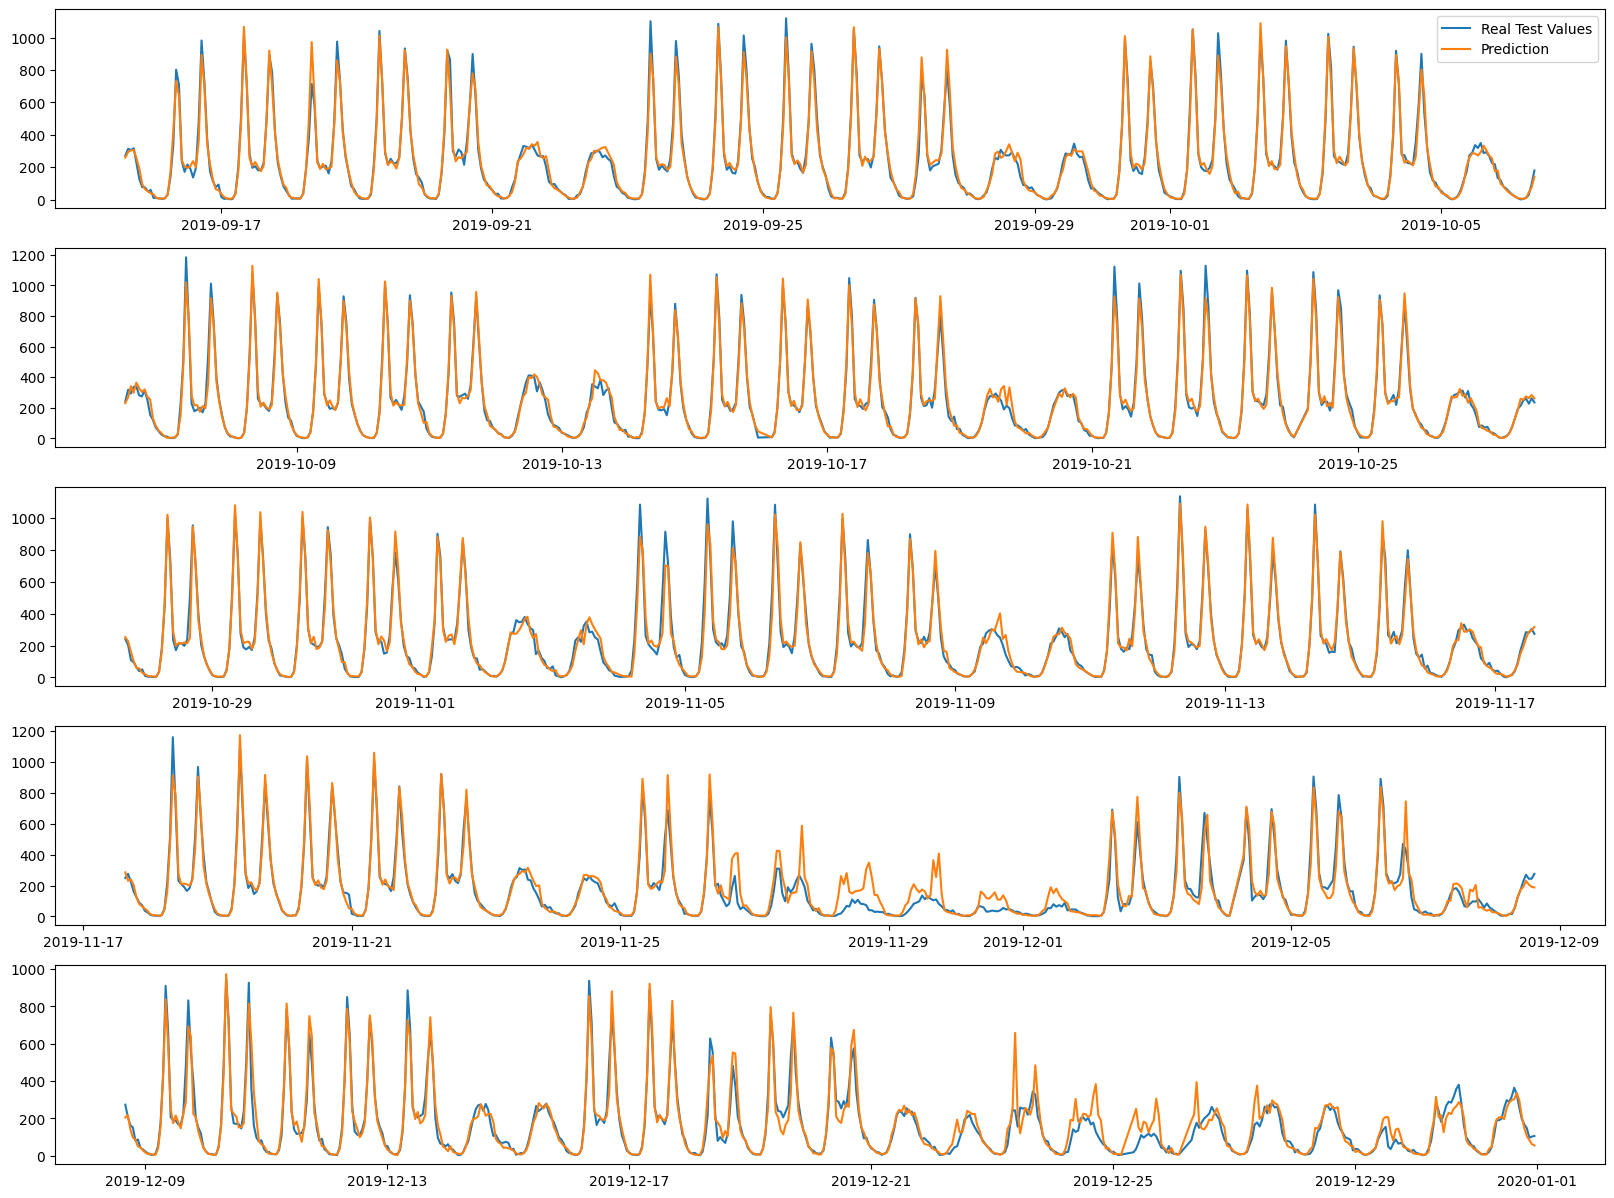
\includegraphics[width=\textwidth]{knn_vs_actual_data.png}
    \caption{Comparison between values predicted by the KNN model and real test values.}
    % \label{fig:png}
\end{figure}

\begin{table}[!ht]
    \centering
    \begin{tabular}{|l|l|l|}
    \hline
        \textbf{Model Name} & \textbf{Unoptimized} & \textbf{Optimized} \\ \hline
        RandomForestRegressor & 0.954284 & 0.954296 \\ \hline
        KNeighborsRegressor & 0.955088 & \textbf{0.956773} \\ \hline
        XGBRFRegressor & 0.946470 & 0.955571 \\ \hline
    \end{tabular}
    \caption{Comparison of the R² value of the different models.}
\end{table}

The most important features for the prediction were found to be the lag values from one week before, as well as the \texttt{is\_workday} feature. Temperature and precipitation were found to have little impact on the prediction. Since K-Nearest Neighbors does not allow feature importance analysis, the values were calculated based on \texttt{XGBRFRegressor} and are show in figure \ref{fig:feature_importance}.

\begin{figure}[hbtp]
    \centering
    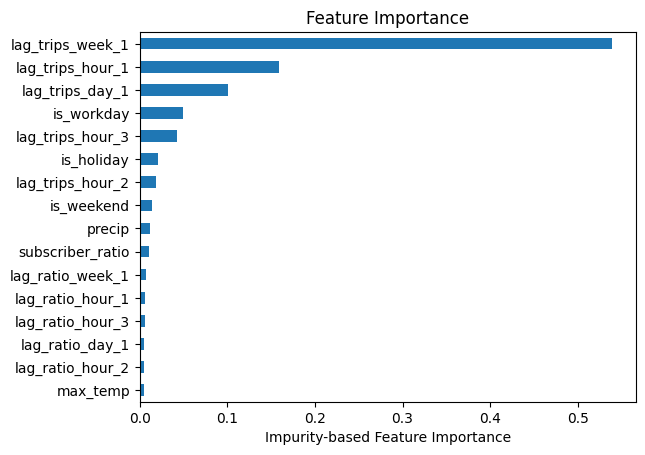
\includegraphics[width=0.7\textwidth]{feature_importance.png}
    \caption{Feature importance as returned by the XGBoost Random Forest Regressor.}
    \label{fig:feature_importance}
\end{figure}

Further improvement could be achieved by using enhanced weather data for the features. The mild climate in San Francisco with low precipitation and temperature ranges allowing riding a bike all year long have a little influence on the demand. Possible enhancements could be achieved through wind strength and direction, since San Francisco's location in a bay area.
 
In case of the selected prediction models, improvements can be achieved by an advanced hyperparameter tuning. Our computational resources are limited, and especially tuning the XGBoost hyperparameters is cost-intensive. For reference, we show a detailed visualization of the effect of hyperparameter tuning  in the appendix \ref{appendix:knn_parameters} (using the KNN model as an example).


\section{Conclusion}

Our goal was to inform and improve business decisions for the bike-sharing platform Lyft. The analysis of the bike-sharing data has provided insights into the temporal and geographical demand patterns, as well as customer and time-based clusters. Based on the findings, it is recommended that Lyft focuses on increasing the availability of bikes at stations located in downtown San Francisco during the weekday morning and evening rush hours, as well as at the docks. Additionally, Lyft should provide promotions and incentives for short-trip customers during the weekdays, and for long-trip customers on weekends. Finally, as bike sharing is a popular option for the 'last mile connectivity' on the customer's way to work, Lyft should consider corporate subscriptions in the B2B market.
The scope of the project was limited to data from only one year of the bike-sharing system, which could be expanded to multiple years to provide more comprehensive findings and analysis of usage and system growth. Additionally, the dataset's features were limited, such as the lack of information on user demographics, which would have allowed for more advanced user clustering and segmentation. In terms of revenue calculation, the results were limited by the fact that revenue calculation for 2019 data was based on the 2023 pricing model. 


% Bibliography
\clearpage
\phantomsection   % Nessecary again, so that the link doesn't point to the conclusion
\addcontentsline{toc}{chapter}{Literatur}
\printbibliography

% Appendix
\begin{appendices}
    
\section{K-nearest Neighbors hyperparameter optimization}\label{appendix:knn_parameters}
This figure shows the importance of different hyperparameters of the K-nearest Neighbors model regarding the R² score.


\begin{figure}[h]
    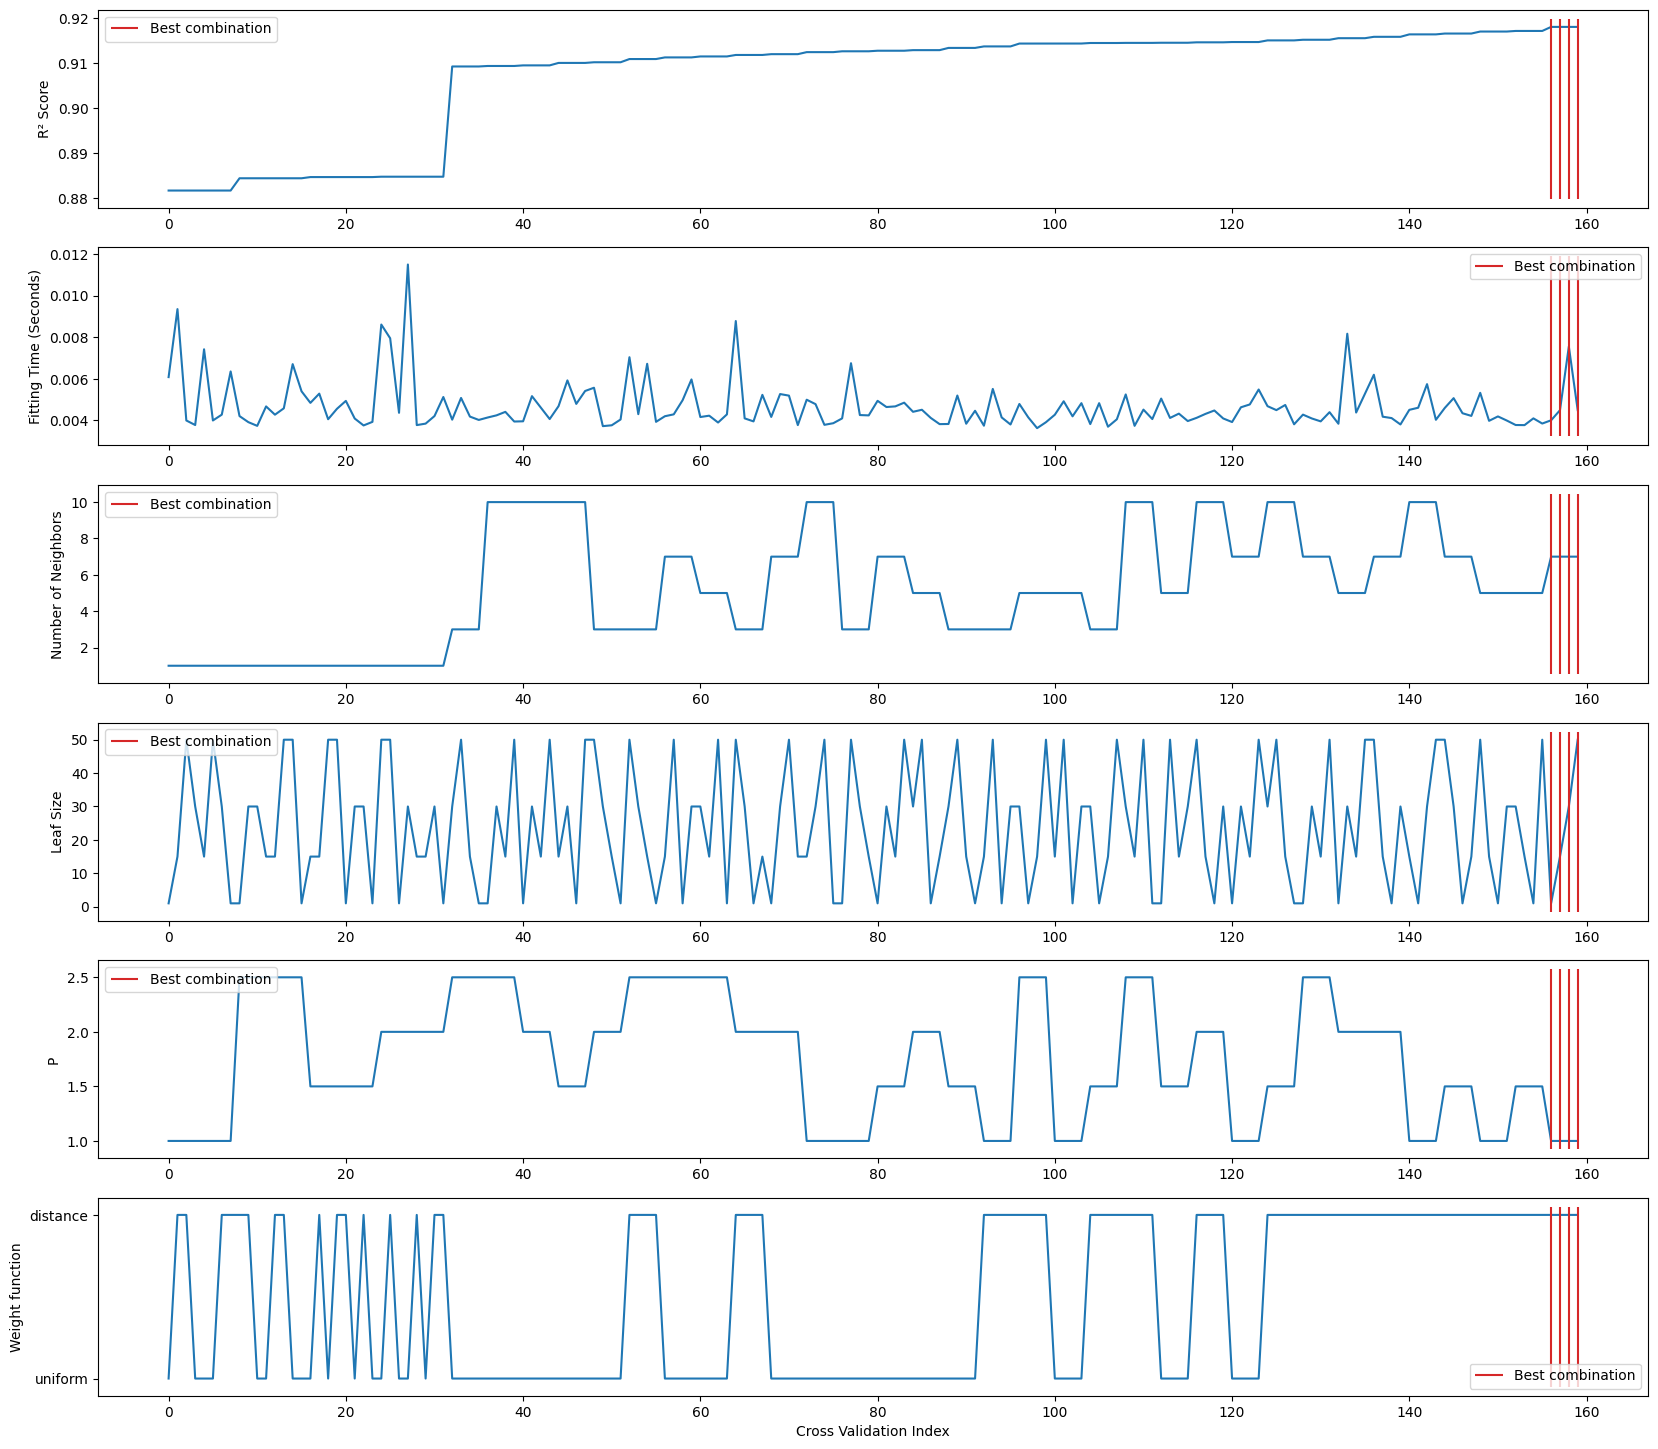
\includegraphics[width=\textwidth]{knn_hyperparameters.png}
    % \label{fig:png}
\end{figure}


\section{Distribution of Work}
We split up on the implementation and documentation between our group members, the following list shows who was mainly involved in which task:

\begin{itemize}
    \item Weather Data Cleaning: Tobias
    \item Bike Data Cleaning: Leo, Manuel
    \item Geo Data Cleaning: Laurenz, Leo, Manuel, Tobias
    \item KPI: Laurenz, Tobias
    \item Descriptive Analytics: Leo, Manuel
    \item Bike and Weather Clustering: Leo
    \item Geo Clustering: Laurenz, Leo, Manuel, Tobias
    \item Predictive Analytics: Leo, Laurenz 
    \item Report: Laurenz, Leo, Manuel, Tobias
\end{itemize}

\end{appendices}


\end{document}
